\documentclass[twoside]{book}

% Packages required by doxygen
\usepackage{fixltx2e}
\usepackage{calc}
\usepackage{doxygen}
\usepackage[export]{adjustbox} % also loads graphicx
\usepackage{graphicx}
\usepackage[utf8]{inputenc}
\usepackage{makeidx}
\usepackage{multicol}
\usepackage{multirow}
\PassOptionsToPackage{warn}{textcomp}
\usepackage{textcomp}
\usepackage[nointegrals]{wasysym}
\usepackage[table]{xcolor}

% Font selection
\usepackage[T1]{fontenc}
\usepackage[scaled=.90]{helvet}
\usepackage{courier}
\usepackage{amssymb}
\usepackage{sectsty}
\renewcommand{\familydefault}{\sfdefault}
\allsectionsfont{%
  \fontseries{bc}\selectfont%
  \color{darkgray}%
}
\renewcommand{\DoxyLabelFont}{%
  \fontseries{bc}\selectfont%
  \color{darkgray}%
}
\newcommand{\+}{\discretionary{\mbox{\scriptsize$\hookleftarrow$}}{}{}}

% Page & text layout
\usepackage{geometry}
\geometry{%
  a4paper,%
  top=2.5cm,%
  bottom=2.5cm,%
  left=2.5cm,%
  right=2.5cm%
}
\tolerance=750
\hfuzz=15pt
\hbadness=750
\setlength{\emergencystretch}{15pt}
\setlength{\parindent}{0cm}
\setlength{\parskip}{3ex plus 2ex minus 2ex}
\makeatletter
\renewcommand{\paragraph}{%
  \@startsection{paragraph}{4}{0ex}{-1.0ex}{1.0ex}{%
    \normalfont\normalsize\bfseries\SS@parafont%
  }%
}
\renewcommand{\subparagraph}{%
  \@startsection{subparagraph}{5}{0ex}{-1.0ex}{1.0ex}{%
    \normalfont\normalsize\bfseries\SS@subparafont%
  }%
}
\makeatother

% Headers & footers
\usepackage{fancyhdr}
\pagestyle{fancyplain}
\fancyhead[LE]{\fancyplain{}{\bfseries\thepage}}
\fancyhead[CE]{\fancyplain{}{}}
\fancyhead[RE]{\fancyplain{}{\bfseries\leftmark}}
\fancyhead[LO]{\fancyplain{}{\bfseries\rightmark}}
\fancyhead[CO]{\fancyplain{}{}}
\fancyhead[RO]{\fancyplain{}{\bfseries\thepage}}
\fancyfoot[LE]{\fancyplain{}{}}
\fancyfoot[CE]{\fancyplain{}{}}
\fancyfoot[RE]{\fancyplain{}{\bfseries\scriptsize Generated by Doxygen }}
\fancyfoot[LO]{\fancyplain{}{\bfseries\scriptsize Generated by Doxygen }}
\fancyfoot[CO]{\fancyplain{}{}}
\fancyfoot[RO]{\fancyplain{}{}}
\renewcommand{\footrulewidth}{0.4pt}
\renewcommand{\chaptermark}[1]{%
  \markboth{#1}{}%
}
\renewcommand{\sectionmark}[1]{%
  \markright{\thesection\ #1}%
}

% Indices & bibliography
\usepackage{natbib}
\usepackage[titles]{tocloft}
\setcounter{tocdepth}{3}
\setcounter{secnumdepth}{5}
\makeindex

% Hyperlinks (required, but should be loaded last)
\usepackage{ifpdf}
\ifpdf
  \usepackage[pdftex,pagebackref=true]{hyperref}
\else
  \usepackage[ps2pdf,pagebackref=true]{hyperref}
\fi
\hypersetup{%
  colorlinks=true,%
  linkcolor=blue,%
  citecolor=blue,%
  unicode%
}

% Custom commands
\newcommand{\clearemptydoublepage}{%
  \newpage{\pagestyle{empty}\cleardoublepage}%
}

\usepackage{caption}
\captionsetup{labelsep=space,justification=centering,font={bf},singlelinecheck=off,skip=4pt,position=top}

%===== C O N T E N T S =====

\begin{document}

% Titlepage & ToC
\hypersetup{pageanchor=false,
             bookmarksnumbered=true,
             pdfencoding=unicode
            }
\pagenumbering{alph}
\begin{titlepage}
\vspace*{7cm}
\begin{center}%
{\Large Laboratorio 2 }\\
\vspace*{1cm}
{\large Generated by Doxygen 1.8.12}\\
\end{center}
\end{titlepage}
\clearemptydoublepage
\pagenumbering{roman}
\tableofcontents
\clearemptydoublepage
\pagenumbering{arabic}
\hypersetup{pageanchor=true}

%--- Begin generated contents ---
\chapter{Hierarchical Index}
\section{Class Hierarchy}
This inheritance list is sorted roughly, but not completely, alphabetically\+:\begin{DoxyCompactList}
\item \contentsline{section}{Figuras}{\pageref{class_figuras}}{}
\begin{DoxyCompactList}
\item \contentsline{section}{Circulo}{\pageref{class_circulo}}{}
\item \contentsline{section}{Cuadrado}{\pageref{class_cuadrado}}{}
\item \contentsline{section}{Triangulo}{\pageref{class_triangulo}}{}
\end{DoxyCompactList}
\end{DoxyCompactList}

\chapter{Class Index}
\section{Class List}
Here are the classes, structs, unions and interfaces with brief descriptions\+:\begin{DoxyCompactList}
\item\contentsline{section}{\hyperlink{classblastobject}{blastobject} }{\pageref{classblastobject}}{}
\end{DoxyCompactList}

\chapter{File Index}
\section{File List}
Here is a list of all documented files with brief descriptions\+:\begin{DoxyCompactList}
\item\contentsline{section}{{\bfseries blastobject.\+h} }{\pageref{blastobject_8h}}{}
\item\contentsline{section}{\hyperlink{main_8cpp}{main.\+cpp} \\*En este programa se utiliza el algoritmo B\+L\+A\+ST para comparacion de secuencias en su version mas simple, comparando con una base de datos creada por el usuario con el proposito de observar su comportamiento de algoritmo y sus resultados. En este caso dichos objetos son del tipo blastobject }{\pageref{main_8cpp}}{}
\end{DoxyCompactList}

\chapter{Class Documentation}
\hypertarget{class_circulo}{}\section{Circulo Class Reference}
\label{class_circulo}\index{Circulo@{Circulo}}


Inheritance diagram for Circulo\+:
\nopagebreak
\begin{figure}[H]
\begin{center}
\leavevmode
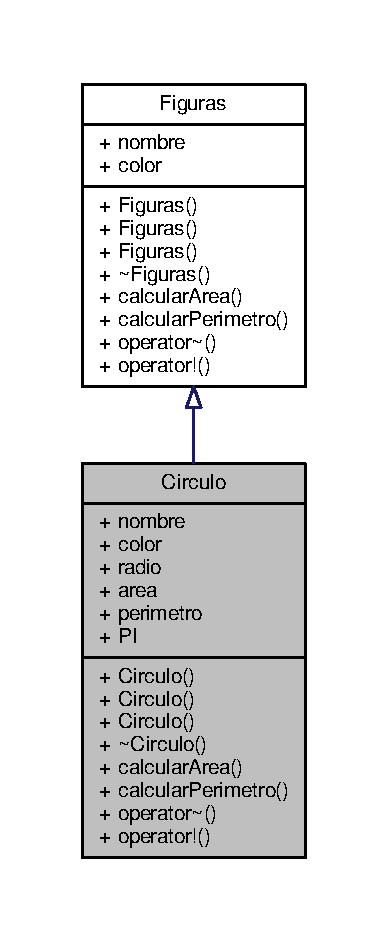
\includegraphics[width=186pt]{class_circulo__inherit__graph}
\end{center}
\end{figure}


Collaboration diagram for Circulo\+:
\nopagebreak
\begin{figure}[H]
\begin{center}
\leavevmode
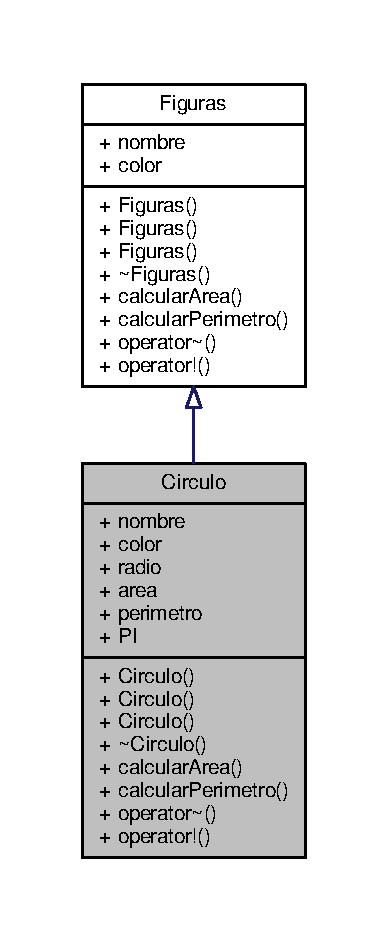
\includegraphics[width=186pt]{class_circulo__coll__graph}
\end{center}
\end{figure}
\subsection*{Public Member Functions}
\begin{DoxyCompactItemize}
\item 
\hypertarget{class_circulo_a6933bf908b78a4167684081a3a8f257f}{}\label{class_circulo_a6933bf908b78a4167684081a3a8f257f} 
\hyperlink{class_circulo_a6933bf908b78a4167684081a3a8f257f}{Circulo} ()
\begin{DoxyCompactList}\small\item\em Constructor vacio de la clase \hyperlink{class_circulo}{Circulo}. \end{DoxyCompactList}\item 
\hyperlink{class_circulo_a14db1f1a04f7adfa9f3e785fce82419c}{Circulo} (string nombre, string color, double radio)
\begin{DoxyCompactList}\small\item\em Constructor sobrecargado de la clase \hyperlink{class_triangulo}{Triangulo}. \end{DoxyCompactList}\item 
\hyperlink{class_circulo_aa1ceac8b166daa79997baa338d6e37e5}{Circulo} (const \hyperlink{class_circulo}{Circulo} \&orig)
\begin{DoxyCompactList}\small\item\em Constructor de la clase \hyperlink{class_circulo}{Circulo}. \end{DoxyCompactList}\item 
\hypertarget{class_circulo_a8efe39e0e89487519cd802f0738d3bf4}{}\label{class_circulo_a8efe39e0e89487519cd802f0738d3bf4} 
virtual \hyperlink{class_circulo_a8efe39e0e89487519cd802f0738d3bf4}{$\sim$\+Circulo} ()
\begin{DoxyCompactList}\small\item\em Destructor de la clase \hyperlink{class_circulo}{Circulo}. \end{DoxyCompactList}\item 
virtual void \hyperlink{class_circulo_a98d2107db46b9f7aacf47a6500a154d5}{calcular\+Area} (double radio)
\begin{DoxyCompactList}\small\item\em Calcula el area del circulo con sus parametros. \end{DoxyCompactList}\item 
virtual void \hyperlink{class_circulo_a4b621679f004d4a093cb18b676079a01}{calcular\+Perimetro} (double radio)
\begin{DoxyCompactList}\small\item\em Calcula el perimetro del circulo con sus parametros. \end{DoxyCompactList}\item 
\hypertarget{class_circulo_a8db226b0c3bad5b8a01d60afb45838c7}{}\label{class_circulo_a8db226b0c3bad5b8a01d60afb45838c7} 
virtual void \hyperlink{class_circulo_a8db226b0c3bad5b8a01d60afb45838c7}{operator$\sim$} ()
\begin{DoxyCompactList}\small\item\em Sobrecarga el operador $\sim$ para imprimir los atributos de la clase. \end{DoxyCompactList}\item 
\hypertarget{class_circulo_a64bd2cabfdbca872d44bf1eb13f59cbb}{}\label{class_circulo_a64bd2cabfdbca872d44bf1eb13f59cbb} 
virtual void \hyperlink{class_circulo_a64bd2cabfdbca872d44bf1eb13f59cbb}{operator!} ()
\begin{DoxyCompactList}\small\item\em Sobrecarga el operador $\sim$ para imprimir los atributos de la clase. \end{DoxyCompactList}\end{DoxyCompactItemize}
\subsection*{Public Attributes}
\begin{DoxyCompactItemize}
\item 
\hypertarget{class_circulo_a4ab11e667cbed98312c5f1688bf486c0}{}\label{class_circulo_a4ab11e667cbed98312c5f1688bf486c0} 
string {\bfseries nombre}
\item 
\hypertarget{class_circulo_a617c127941b509f6265ab59c141d7fea}{}\label{class_circulo_a617c127941b509f6265ab59c141d7fea} 
string {\bfseries color}
\item 
\hypertarget{class_circulo_aba57029c5768d344c4ef536e5323122b}{}\label{class_circulo_aba57029c5768d344c4ef536e5323122b} 
double {\bfseries radio}
\item 
\hypertarget{class_circulo_aad66b63b8596c7a11984529187ce735b}{}\label{class_circulo_aad66b63b8596c7a11984529187ce735b} 
double {\bfseries area}
\item 
\hypertarget{class_circulo_abb3ea097fcf69731319dbae8ddb21235}{}\label{class_circulo_abb3ea097fcf69731319dbae8ddb21235} 
double {\bfseries perimetro}
\item 
\hypertarget{class_circulo_a15eb99a8a0c6af955085b14baf8a35c1}{}\label{class_circulo_a15eb99a8a0c6af955085b14baf8a35c1} 
const double {\bfseries PI} = 3.\+141592653589793238463
\end{DoxyCompactItemize}


\subsection{Constructor \& Destructor Documentation}
\hypertarget{class_circulo_a14db1f1a04f7adfa9f3e785fce82419c}{}\label{class_circulo_a14db1f1a04f7adfa9f3e785fce82419c} 
\index{Circulo@{Circulo}!Circulo@{Circulo}}
\index{Circulo@{Circulo}!Circulo@{Circulo}}
\subsubsection{\texorpdfstring{Circulo()}{Circulo()}\hspace{0.1cm}{\footnotesize\ttfamily [1/2]}}
{\ttfamily Circulo\+::\+Circulo (\begin{DoxyParamCaption}\item[{string}]{nombre,  }\item[{string}]{color,  }\item[{double}]{radio }\end{DoxyParamCaption})}



Constructor sobrecargado de la clase \hyperlink{class_triangulo}{Triangulo}. 


\begin{DoxyParams}{Parameters}
{\em nombre} & Nombre de la figura. \\
\hline
{\em color} & Color de la figura. \\
\hline
{\em radio} & Valor del radio de la figura. \\
\hline
\end{DoxyParams}
\hypertarget{class_circulo_aa1ceac8b166daa79997baa338d6e37e5}{}\label{class_circulo_aa1ceac8b166daa79997baa338d6e37e5} 
\index{Circulo@{Circulo}!Circulo@{Circulo}}
\index{Circulo@{Circulo}!Circulo@{Circulo}}
\subsubsection{\texorpdfstring{Circulo()}{Circulo()}\hspace{0.1cm}{\footnotesize\ttfamily [2/2]}}
{\ttfamily Circulo\+::\+Circulo (\begin{DoxyParamCaption}\item[{const \hyperlink{class_circulo}{Circulo} \&}]{orig }\end{DoxyParamCaption})}



Constructor de la clase \hyperlink{class_circulo}{Circulo}. 


\begin{DoxyParams}{Parameters}
{\em Circulo\&} & Constante objeto. \\
\hline
\end{DoxyParams}


\subsection{Member Function Documentation}
\hypertarget{class_circulo_a98d2107db46b9f7aacf47a6500a154d5}{}\label{class_circulo_a98d2107db46b9f7aacf47a6500a154d5} 
\index{Circulo@{Circulo}!calcular\+Area@{calcular\+Area}}
\index{calcular\+Area@{calcular\+Area}!Circulo@{Circulo}}
\subsubsection{\texorpdfstring{calcular\+Area()}{calcularArea()}}
{\ttfamily void Circulo\+::calcular\+Area (\begin{DoxyParamCaption}\item[{double}]{radio }\end{DoxyParamCaption})\hspace{0.3cm}{\ttfamily [virtual]}}



Calcula el area del circulo con sus parametros. 


\begin{DoxyParams}{Parameters}
{\em radio} & Valor del radio de la figura. \\
\hline
\end{DoxyParams}
\hypertarget{class_circulo_a4b621679f004d4a093cb18b676079a01}{}\label{class_circulo_a4b621679f004d4a093cb18b676079a01} 
\index{Circulo@{Circulo}!calcular\+Perimetro@{calcular\+Perimetro}}
\index{calcular\+Perimetro@{calcular\+Perimetro}!Circulo@{Circulo}}
\subsubsection{\texorpdfstring{calcular\+Perimetro()}{calcularPerimetro()}}
{\ttfamily void Circulo\+::calcular\+Perimetro (\begin{DoxyParamCaption}\item[{double}]{radio }\end{DoxyParamCaption})\hspace{0.3cm}{\ttfamily [virtual]}}



Calcula el perimetro del circulo con sus parametros. 


\begin{DoxyParams}{Parameters}
{\em radio} & Valor del radio de la figura. \\
\hline
\end{DoxyParams}


The documentation for this class was generated from the following files\+:\begin{DoxyCompactItemize}
\item 
Figuras.\+h\item 
Figuras.\+cpp\end{DoxyCompactItemize}

\hypertarget{class_cuadrado}{}\section{Cuadrado Class Reference}
\label{class_cuadrado}\index{Cuadrado@{Cuadrado}}


Inheritance diagram for Cuadrado\+:
\nopagebreak
\begin{figure}[H]
\begin{center}
\leavevmode
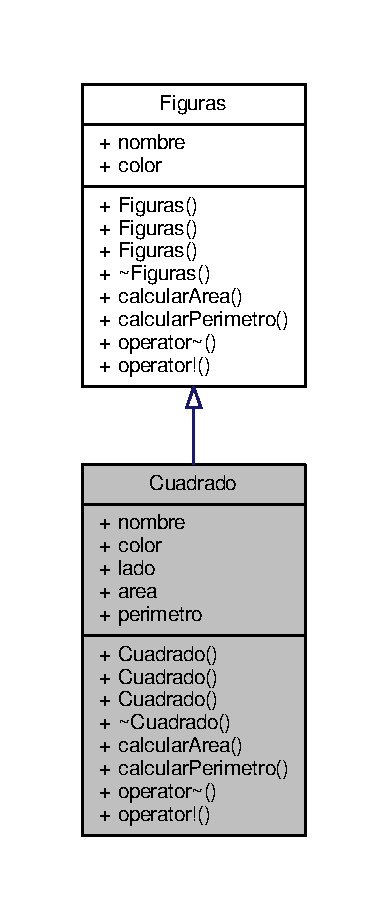
\includegraphics[width=186pt]{class_cuadrado__inherit__graph}
\end{center}
\end{figure}


Collaboration diagram for Cuadrado\+:
\nopagebreak
\begin{figure}[H]
\begin{center}
\leavevmode
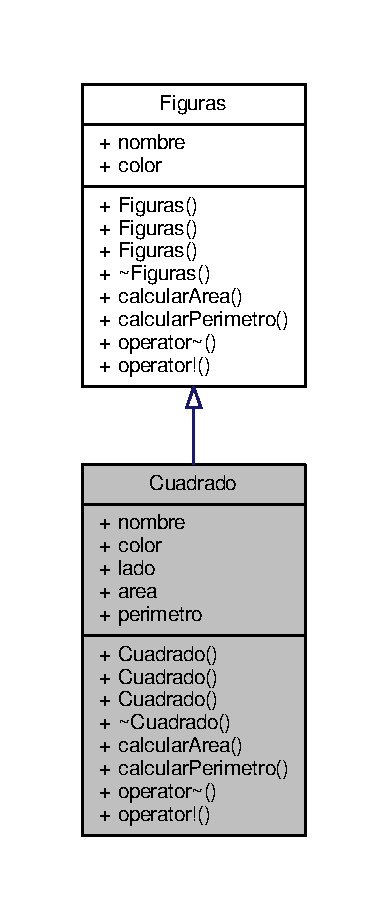
\includegraphics[width=186pt]{class_cuadrado__coll__graph}
\end{center}
\end{figure}
\subsection*{Public Member Functions}
\begin{DoxyCompactItemize}
\item 
\hypertarget{class_cuadrado_ad28d9dddc29e1987ec620b07b0a4acc9}{}\label{class_cuadrado_ad28d9dddc29e1987ec620b07b0a4acc9} 
\hyperlink{class_cuadrado_ad28d9dddc29e1987ec620b07b0a4acc9}{Cuadrado} ()
\begin{DoxyCompactList}\small\item\em Constructor vacio de la clase \hyperlink{class_cuadrado}{Cuadrado}. \end{DoxyCompactList}\item 
\hyperlink{class_cuadrado_afb489ccf7f7b4e2837d080bee5f6656a}{Cuadrado} (string nombre, string color, double lado)
\begin{DoxyCompactList}\small\item\em Constructor sobrecargado de la clase \hyperlink{class_cuadrado}{Cuadrado}. \end{DoxyCompactList}\item 
\hyperlink{class_cuadrado_a51f15bc1eb52008d394ac1191e257aeb}{Cuadrado} (const \hyperlink{class_cuadrado}{Cuadrado} \&orig)
\begin{DoxyCompactList}\small\item\em Constructor de la clase \hyperlink{class_cuadrado}{Cuadrado}. \end{DoxyCompactList}\item 
\hypertarget{class_cuadrado_a9f5bf29c9b8368ad45a4a3c12f9fd7c2}{}\label{class_cuadrado_a9f5bf29c9b8368ad45a4a3c12f9fd7c2} 
virtual \hyperlink{class_cuadrado_a9f5bf29c9b8368ad45a4a3c12f9fd7c2}{$\sim$\+Cuadrado} ()
\begin{DoxyCompactList}\small\item\em Destructor de la clase \hyperlink{class_cuadrado}{Cuadrado}. \end{DoxyCompactList}\item 
\hypertarget{class_cuadrado_a21bd92e4d2fa822d898a1a70100012ec}{}\label{class_cuadrado_a21bd92e4d2fa822d898a1a70100012ec} 
virtual void \hyperlink{class_cuadrado_a21bd92e4d2fa822d898a1a70100012ec}{calcular\+Area} (double lado)
\begin{DoxyCompactList}\small\item\em Llama a la funcion en la clase \hyperlink{class_figuras}{Figuras}. \end{DoxyCompactList}\item 
\hypertarget{class_cuadrado_a2deca0b349c2f70d771282c75e737c0c}{}\label{class_cuadrado_a2deca0b349c2f70d771282c75e737c0c} 
virtual void \hyperlink{class_cuadrado_a2deca0b349c2f70d771282c75e737c0c}{calcular\+Perimetro} (double lado)
\begin{DoxyCompactList}\small\item\em Llama a la funcion en la clase \hyperlink{class_figuras}{Figuras}. \end{DoxyCompactList}\item 
\hypertarget{class_cuadrado_a6303f81de8d357f415d00a116b73a6fc}{}\label{class_cuadrado_a6303f81de8d357f415d00a116b73a6fc} 
virtual void \hyperlink{class_cuadrado_a6303f81de8d357f415d00a116b73a6fc}{operator$\sim$} ()
\begin{DoxyCompactList}\small\item\em Sobrecarga el operador $\sim$ para imprimir los atributos de la clase. \end{DoxyCompactList}\item 
\hypertarget{class_cuadrado_a78be5dcef640ad7f82858f44fb623af5}{}\label{class_cuadrado_a78be5dcef640ad7f82858f44fb623af5} 
virtual void \hyperlink{class_cuadrado_a78be5dcef640ad7f82858f44fb623af5}{operator!} ()
\begin{DoxyCompactList}\small\item\em Sobrecarga el operador ! para imprimir los calculos de la clase. \end{DoxyCompactList}\end{DoxyCompactItemize}
\subsection*{Public Attributes}
\begin{DoxyCompactItemize}
\item 
\hypertarget{class_cuadrado_a2d85cc9025c27709524fff4f8ee89645}{}\label{class_cuadrado_a2d85cc9025c27709524fff4f8ee89645} 
string {\bfseries nombre}
\item 
\hypertarget{class_cuadrado_ae8ad3499e4f99746dde86b42b3e50c2d}{}\label{class_cuadrado_ae8ad3499e4f99746dde86b42b3e50c2d} 
string {\bfseries color}
\item 
\hypertarget{class_cuadrado_a0480679f3e1c059282f532167c81d439}{}\label{class_cuadrado_a0480679f3e1c059282f532167c81d439} 
double {\bfseries lado}
\item 
\hypertarget{class_cuadrado_a5912fed1157e6e738bca7477013a3699}{}\label{class_cuadrado_a5912fed1157e6e738bca7477013a3699} 
double {\bfseries area}
\item 
\hypertarget{class_cuadrado_aabf689b756dda0bd3f3b09e021080113}{}\label{class_cuadrado_aabf689b756dda0bd3f3b09e021080113} 
double {\bfseries perimetro}
\end{DoxyCompactItemize}


\subsection{Constructor \& Destructor Documentation}
\hypertarget{class_cuadrado_afb489ccf7f7b4e2837d080bee5f6656a}{}\label{class_cuadrado_afb489ccf7f7b4e2837d080bee5f6656a} 
\index{Cuadrado@{Cuadrado}!Cuadrado@{Cuadrado}}
\index{Cuadrado@{Cuadrado}!Cuadrado@{Cuadrado}}
\subsubsection{\texorpdfstring{Cuadrado()}{Cuadrado()}\hspace{0.1cm}{\footnotesize\ttfamily [1/2]}}
{\ttfamily Cuadrado\+::\+Cuadrado (\begin{DoxyParamCaption}\item[{string}]{nombre,  }\item[{string}]{color,  }\item[{double}]{lado }\end{DoxyParamCaption})}



Constructor sobrecargado de la clase \hyperlink{class_cuadrado}{Cuadrado}. 


\begin{DoxyParams}{Parameters}
{\em nombre} & Nombre de la figura. \\
\hline
{\em color} & Color de la figura. \\
\hline
{\em lado} & Valor del lado de la figura. \\
\hline
\end{DoxyParams}
\hypertarget{class_cuadrado_a51f15bc1eb52008d394ac1191e257aeb}{}\label{class_cuadrado_a51f15bc1eb52008d394ac1191e257aeb} 
\index{Cuadrado@{Cuadrado}!Cuadrado@{Cuadrado}}
\index{Cuadrado@{Cuadrado}!Cuadrado@{Cuadrado}}
\subsubsection{\texorpdfstring{Cuadrado()}{Cuadrado()}\hspace{0.1cm}{\footnotesize\ttfamily [2/2]}}
{\ttfamily Cuadrado\+::\+Cuadrado (\begin{DoxyParamCaption}\item[{const \hyperlink{class_cuadrado}{Cuadrado} \&}]{orig }\end{DoxyParamCaption})}



Constructor de la clase \hyperlink{class_cuadrado}{Cuadrado}. 


\begin{DoxyParams}{Parameters}
{\em Cuadrado\&} & Constante objeto. \\
\hline
\end{DoxyParams}


The documentation for this class was generated from the following files\+:\begin{DoxyCompactItemize}
\item 
Figuras.\+h\item 
Figuras.\+cpp\end{DoxyCompactItemize}

\hypertarget{class_figuras}{}\section{Figuras Class Reference}
\label{class_figuras}\index{Figuras@{Figuras}}


Inheritance diagram for Figuras\+:
\nopagebreak
\begin{figure}[H]
\begin{center}
\leavevmode
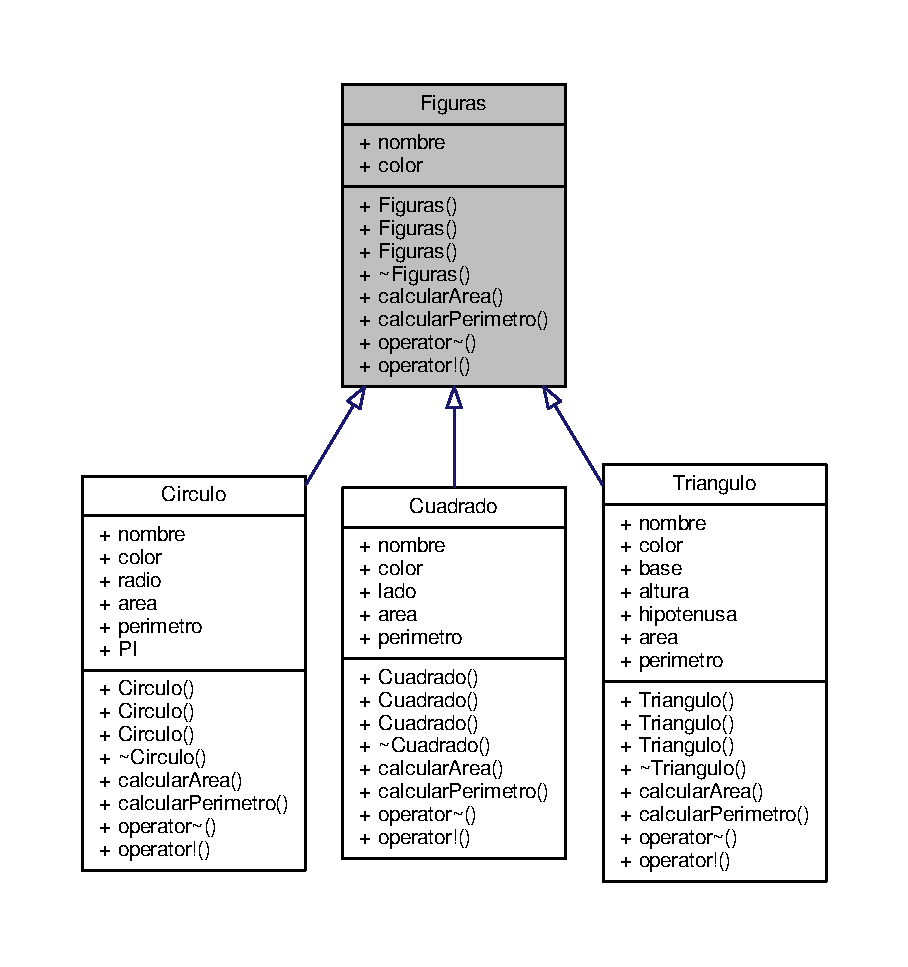
\includegraphics[width=350pt]{class_figuras__inherit__graph}
\end{center}
\end{figure}


Collaboration diagram for Figuras\+:
\nopagebreak
\begin{figure}[H]
\begin{center}
\leavevmode
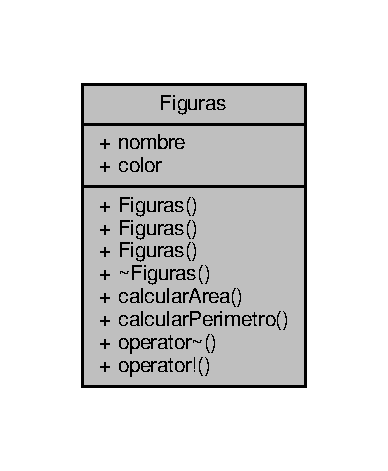
\includegraphics[width=186pt]{class_figuras__coll__graph}
\end{center}
\end{figure}
\subsection*{Public Member Functions}
\begin{DoxyCompactItemize}
\item 
\hypertarget{class_figuras_aa4a6b2a853e7370ae3085650eb4ba54c}{}\label{class_figuras_aa4a6b2a853e7370ae3085650eb4ba54c} 
\hyperlink{class_figuras_aa4a6b2a853e7370ae3085650eb4ba54c}{Figuras} ()
\begin{DoxyCompactList}\small\item\em Constructor vacio de clase \hyperlink{class_figuras}{Figuras}. \end{DoxyCompactList}\item 
\hyperlink{class_figuras_aa27ab1cfbd67dc1d7b806065586875f7}{Figuras} (string nombre, string color)
\begin{DoxyCompactList}\small\item\em Constructor sobrecargado de la clase \hyperlink{class_figuras}{Figuras}. \end{DoxyCompactList}\item 
\hyperlink{class_figuras_aa5cb44be3f36d79786b13fc8d9a7da7f}{Figuras} (const \hyperlink{class_figuras}{Figuras} \&orig)
\begin{DoxyCompactList}\small\item\em Constructor de la clase \hyperlink{class_figuras}{Figuras}. \end{DoxyCompactList}\item 
\hypertarget{class_figuras_a3c630ab1c3c75dd98f38a4e30e7820f2}{}\label{class_figuras_a3c630ab1c3c75dd98f38a4e30e7820f2} 
virtual \hyperlink{class_figuras_a3c630ab1c3c75dd98f38a4e30e7820f2}{$\sim$\+Figuras} ()
\begin{DoxyCompactList}\small\item\em Destructor de la clase \hyperlink{class_figuras}{Figuras}. \end{DoxyCompactList}\item 
\hypertarget{class_figuras_aab7794256f0f226206b840b8668babfe}{}\label{class_figuras_aab7794256f0f226206b840b8668babfe} 
virtual void \hyperlink{class_figuras_aab7794256f0f226206b840b8668babfe}{calcular\+Area} ()
\begin{DoxyCompactList}\small\item\em Llama a la funcion en la clase \hyperlink{class_figuras}{Figuras}. \end{DoxyCompactList}\item 
\hypertarget{class_figuras_a90c8e15e0a6a982baa363bff28d4774d}{}\label{class_figuras_a90c8e15e0a6a982baa363bff28d4774d} 
virtual void \hyperlink{class_figuras_a90c8e15e0a6a982baa363bff28d4774d}{calcular\+Perimetro} ()
\begin{DoxyCompactList}\small\item\em Llama a la funcion en la clase \hyperlink{class_figuras}{Figuras}. \end{DoxyCompactList}\item 
\hypertarget{class_figuras_aa5b277011447abd9b97f305f71635077}{}\label{class_figuras_aa5b277011447abd9b97f305f71635077} 
virtual void \hyperlink{class_figuras_aa5b277011447abd9b97f305f71635077}{operator$\sim$} ()
\begin{DoxyCompactList}\small\item\em Sobrecarga el operador $\sim$ para imprimir los atributos de la clase. \end{DoxyCompactList}\item 
\hypertarget{class_figuras_a71c13069c91f1613b77e5d761a7598e7}{}\label{class_figuras_a71c13069c91f1613b77e5d761a7598e7} 
virtual void \hyperlink{class_figuras_a71c13069c91f1613b77e5d761a7598e7}{operator!} ()
\begin{DoxyCompactList}\small\item\em Sobrecarga el operador ! para imprimir los calculos de la clase. \end{DoxyCompactList}\end{DoxyCompactItemize}
\subsection*{Public Attributes}
\begin{DoxyCompactItemize}
\item 
\hypertarget{class_figuras_a88b1e8e830f6810b4bafabfe081ba8ec}{}\label{class_figuras_a88b1e8e830f6810b4bafabfe081ba8ec} 
string {\bfseries nombre}
\item 
\hypertarget{class_figuras_af1980b3c371490afbd9d986748c70b25}{}\label{class_figuras_af1980b3c371490afbd9d986748c70b25} 
string {\bfseries color}
\end{DoxyCompactItemize}


\subsection{Constructor \& Destructor Documentation}
\hypertarget{class_figuras_aa27ab1cfbd67dc1d7b806065586875f7}{}\label{class_figuras_aa27ab1cfbd67dc1d7b806065586875f7} 
\index{Figuras@{Figuras}!Figuras@{Figuras}}
\index{Figuras@{Figuras}!Figuras@{Figuras}}
\subsubsection{\texorpdfstring{Figuras()}{Figuras()}\hspace{0.1cm}{\footnotesize\ttfamily [1/2]}}
{\ttfamily Figuras\+::\+Figuras (\begin{DoxyParamCaption}\item[{string}]{nombre,  }\item[{string}]{color }\end{DoxyParamCaption})}



Constructor sobrecargado de la clase \hyperlink{class_figuras}{Figuras}. 


\begin{DoxyParams}{Parameters}
{\em nombre} & Nombre de la figura. \\
\hline
{\em color} & Color de la figura. \\
\hline
\end{DoxyParams}
\hypertarget{class_figuras_aa5cb44be3f36d79786b13fc8d9a7da7f}{}\label{class_figuras_aa5cb44be3f36d79786b13fc8d9a7da7f} 
\index{Figuras@{Figuras}!Figuras@{Figuras}}
\index{Figuras@{Figuras}!Figuras@{Figuras}}
\subsubsection{\texorpdfstring{Figuras()}{Figuras()}\hspace{0.1cm}{\footnotesize\ttfamily [2/2]}}
{\ttfamily Figuras\+::\+Figuras (\begin{DoxyParamCaption}\item[{const \hyperlink{class_figuras}{Figuras} \&}]{orig }\end{DoxyParamCaption})}



Constructor de la clase \hyperlink{class_figuras}{Figuras}. 


\begin{DoxyParams}{Parameters}
{\em Figuras\&} & Constante objeto. \\
\hline
\end{DoxyParams}


The documentation for this class was generated from the following files\+:\begin{DoxyCompactItemize}
\item 
Figuras.\+h\item 
Figuras.\+cpp\end{DoxyCompactItemize}

\hypertarget{class_triangulo}{}\section{Triangulo Class Reference}
\label{class_triangulo}\index{Triangulo@{Triangulo}}


Inheritance diagram for Triangulo\+:
\nopagebreak
\begin{figure}[H]
\begin{center}
\leavevmode
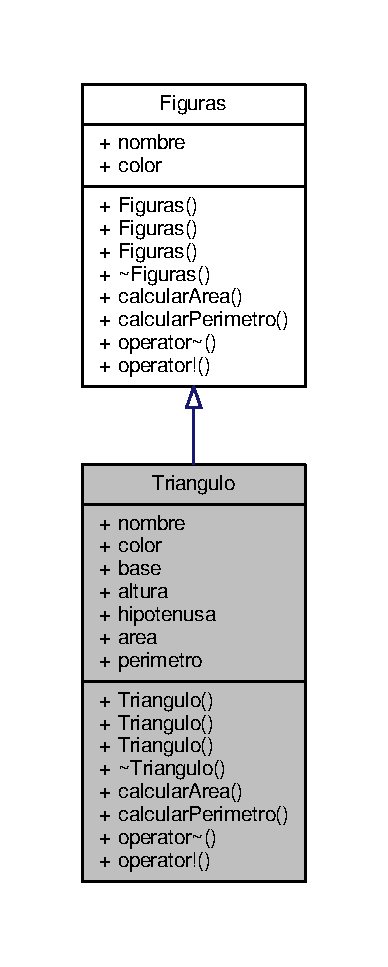
\includegraphics[width=186pt]{class_triangulo__inherit__graph}
\end{center}
\end{figure}


Collaboration diagram for Triangulo\+:
\nopagebreak
\begin{figure}[H]
\begin{center}
\leavevmode
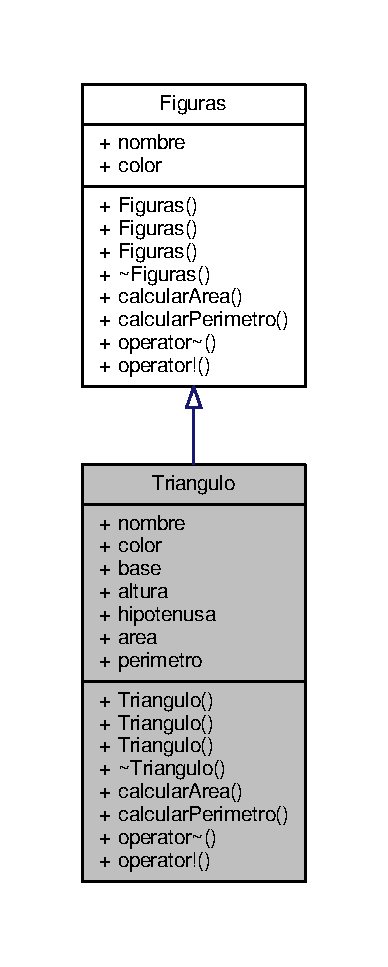
\includegraphics[width=186pt]{class_triangulo__coll__graph}
\end{center}
\end{figure}
\subsection*{Public Member Functions}
\begin{DoxyCompactItemize}
\item 
\hypertarget{class_triangulo_a905d421bd19655a979ccad9e2998db0c}{}\label{class_triangulo_a905d421bd19655a979ccad9e2998db0c} 
\hyperlink{class_triangulo_a905d421bd19655a979ccad9e2998db0c}{Triangulo} ()
\begin{DoxyCompactList}\small\item\em Constructor vacio de la clase \hyperlink{class_triangulo}{Triangulo}. \end{DoxyCompactList}\item 
\hyperlink{class_triangulo_ae8f507a390e27552f82f6fa232120372}{Triangulo} (string nombre, string color, double base, double altura, double hipotenusa)
\begin{DoxyCompactList}\small\item\em Constructor sobrecargado de la clase \hyperlink{class_triangulo}{Triangulo}. \end{DoxyCompactList}\item 
\hyperlink{class_triangulo_a1a7267ad3feb850a9718002420fc2fd8}{Triangulo} (const \hyperlink{class_triangulo}{Triangulo} \&orig)
\begin{DoxyCompactList}\small\item\em Constructor de la clase \hyperlink{class_triangulo}{Triangulo}. \end{DoxyCompactList}\item 
\hypertarget{class_triangulo_aca2be15b19831e8d7a5331808f5c1958}{}\label{class_triangulo_aca2be15b19831e8d7a5331808f5c1958} 
virtual \hyperlink{class_triangulo_aca2be15b19831e8d7a5331808f5c1958}{$\sim$\+Triangulo} ()
\begin{DoxyCompactList}\small\item\em Destructor de la clase \hyperlink{class_cuadrado}{Cuadrado}. \end{DoxyCompactList}\item 
virtual void \hyperlink{class_triangulo_a11f6635bf56a065274b6777f897909e8}{calcular\+Area} (double base, double altura)
\begin{DoxyCompactList}\small\item\em Calcula el area del triangulo con sus parametros. \end{DoxyCompactList}\item 
void \hyperlink{class_triangulo_a76867bdb3344be0d36d76027b810b64f}{calcular\+Perimetro} (double base, double altura, double hipotenusa)
\begin{DoxyCompactList}\small\item\em Calcula el perimetro del triangulo con sus parametros. \end{DoxyCompactList}\item 
\hypertarget{class_triangulo_af7fc480161706ec74ece32e9ef1fed7f}{}\label{class_triangulo_af7fc480161706ec74ece32e9ef1fed7f} 
virtual void \hyperlink{class_triangulo_af7fc480161706ec74ece32e9ef1fed7f}{operator$\sim$} ()
\begin{DoxyCompactList}\small\item\em Sobrecarga el operador $\sim$ para imprimir los atributos de la clase. \end{DoxyCompactList}\item 
\hypertarget{class_triangulo_ae0552ffa9641d36e1f571349e5de1070}{}\label{class_triangulo_ae0552ffa9641d36e1f571349e5de1070} 
virtual void \hyperlink{class_triangulo_ae0552ffa9641d36e1f571349e5de1070}{operator!} ()
\begin{DoxyCompactList}\small\item\em Sobrecarga el operador ! para imprimir los calculos de la clase. \end{DoxyCompactList}\end{DoxyCompactItemize}
\subsection*{Public Attributes}
\begin{DoxyCompactItemize}
\item 
\hypertarget{class_triangulo_a92bbfa4ca7bc38489e7bddd797a84cbf}{}\label{class_triangulo_a92bbfa4ca7bc38489e7bddd797a84cbf} 
string {\bfseries nombre}
\item 
\hypertarget{class_triangulo_a437071d8f69923add54c5bedb74cce10}{}\label{class_triangulo_a437071d8f69923add54c5bedb74cce10} 
string {\bfseries color}
\item 
\hypertarget{class_triangulo_a77fe2a9ef9624495cd93f306ee115e54}{}\label{class_triangulo_a77fe2a9ef9624495cd93f306ee115e54} 
double {\bfseries base}
\item 
\hypertarget{class_triangulo_a4a3435a7e19354df87419f17c9ce309f}{}\label{class_triangulo_a4a3435a7e19354df87419f17c9ce309f} 
double {\bfseries altura}
\item 
\hypertarget{class_triangulo_afbe83fdbbfaf050a12c78fd29f1729f3}{}\label{class_triangulo_afbe83fdbbfaf050a12c78fd29f1729f3} 
double {\bfseries hipotenusa}
\item 
\hypertarget{class_triangulo_a7c272d5536b605370cb7ecd8a0c26d08}{}\label{class_triangulo_a7c272d5536b605370cb7ecd8a0c26d08} 
double {\bfseries area}
\item 
\hypertarget{class_triangulo_afb3326a460dc259a32bddb59cdc106a4}{}\label{class_triangulo_afb3326a460dc259a32bddb59cdc106a4} 
double {\bfseries perimetro}
\end{DoxyCompactItemize}


\subsection{Constructor \& Destructor Documentation}
\hypertarget{class_triangulo_ae8f507a390e27552f82f6fa232120372}{}\label{class_triangulo_ae8f507a390e27552f82f6fa232120372} 
\index{Triangulo@{Triangulo}!Triangulo@{Triangulo}}
\index{Triangulo@{Triangulo}!Triangulo@{Triangulo}}
\subsubsection{\texorpdfstring{Triangulo()}{Triangulo()}\hspace{0.1cm}{\footnotesize\ttfamily [1/2]}}
{\ttfamily Triangulo\+::\+Triangulo (\begin{DoxyParamCaption}\item[{string}]{nombre,  }\item[{string}]{color,  }\item[{double}]{base,  }\item[{double}]{altura,  }\item[{double}]{hipotenusa }\end{DoxyParamCaption})}



Constructor sobrecargado de la clase \hyperlink{class_triangulo}{Triangulo}. 


\begin{DoxyParams}{Parameters}
{\em nombre} & Nombre de la figura. \\
\hline
{\em color} & Color de la figura. \\
\hline
{\em base} & Valor de la base de la figura. \\
\hline
{\em altura} & Valor de la altura de la figura. \\
\hline
{\em hipotenusa} & Valor de la hipotenusa de la figura. \\
\hline
\end{DoxyParams}
\hypertarget{class_triangulo_a1a7267ad3feb850a9718002420fc2fd8}{}\label{class_triangulo_a1a7267ad3feb850a9718002420fc2fd8} 
\index{Triangulo@{Triangulo}!Triangulo@{Triangulo}}
\index{Triangulo@{Triangulo}!Triangulo@{Triangulo}}
\subsubsection{\texorpdfstring{Triangulo()}{Triangulo()}\hspace{0.1cm}{\footnotesize\ttfamily [2/2]}}
{\ttfamily Triangulo\+::\+Triangulo (\begin{DoxyParamCaption}\item[{const \hyperlink{class_triangulo}{Triangulo} \&}]{orig }\end{DoxyParamCaption})}



Constructor de la clase \hyperlink{class_triangulo}{Triangulo}. 


\begin{DoxyParams}{Parameters}
{\em Triangulo\&} & Constante objeto. \\
\hline
\end{DoxyParams}


\subsection{Member Function Documentation}
\hypertarget{class_triangulo_a11f6635bf56a065274b6777f897909e8}{}\label{class_triangulo_a11f6635bf56a065274b6777f897909e8} 
\index{Triangulo@{Triangulo}!calcular\+Area@{calcular\+Area}}
\index{calcular\+Area@{calcular\+Area}!Triangulo@{Triangulo}}
\subsubsection{\texorpdfstring{calcular\+Area()}{calcularArea()}}
{\ttfamily void Triangulo\+::calcular\+Area (\begin{DoxyParamCaption}\item[{double}]{base,  }\item[{double}]{altura }\end{DoxyParamCaption})\hspace{0.3cm}{\ttfamily [virtual]}}



Calcula el area del triangulo con sus parametros. 


\begin{DoxyParams}{Parameters}
{\em base} & Valor de la base de la figura. \\
\hline
{\em altura} & Valor de la altura de la figura. \\
\hline
\end{DoxyParams}
\hypertarget{class_triangulo_a76867bdb3344be0d36d76027b810b64f}{}\label{class_triangulo_a76867bdb3344be0d36d76027b810b64f} 
\index{Triangulo@{Triangulo}!calcular\+Perimetro@{calcular\+Perimetro}}
\index{calcular\+Perimetro@{calcular\+Perimetro}!Triangulo@{Triangulo}}
\subsubsection{\texorpdfstring{calcular\+Perimetro()}{calcularPerimetro()}}
{\ttfamily void Triangulo\+::calcular\+Perimetro (\begin{DoxyParamCaption}\item[{double}]{base,  }\item[{double}]{altura,  }\item[{double}]{hipotenusa }\end{DoxyParamCaption})}



Calcula el perimetro del triangulo con sus parametros. 


\begin{DoxyParams}{Parameters}
{\em base} & Valor de la base de la figura. \\
\hline
{\em altura} & Valor de la altura de la figura. \\
\hline
{\em hipotenusa} & Valor de la hipotenusa de la figura. \\
\hline
\end{DoxyParams}


The documentation for this class was generated from the following files\+:\begin{DoxyCompactItemize}
\item 
Figuras.\+h\item 
Figuras.\+cpp\end{DoxyCompactItemize}

\chapter{File Documentation}
\section{main.\+cpp File Reference}
\label{main_8cpp}\index{main.\+cpp@{main.\+cpp}}


Se implementa la estructura abstracta de grafo usando la matriz de adyacecia y las búsquedas de profundidad y ancho.  


{\ttfamily \#include \char`\"{}Graph.\+h\char`\"{}}\newline
\subsection*{Functions}
\begin{DoxyCompactItemize}
\item 
\label{main_8cpp_ae66f6b31b5ad750f1fe042a706a4e3d4} 
int {\bfseries main} ()
\end{DoxyCompactItemize}


\subsection{Detailed Description}
Se implementa la estructura abstracta de grafo usando la matriz de adyacecia y las búsquedas de profundidad y ancho. 

\begin{DoxyAuthor}{Author}
Jose Fernando Gonzalez Salas \& Isaac Gomez Sanchez 
\end{DoxyAuthor}
\begin{DoxyDate}{Date}
13 de noviembre, 2016 
\end{DoxyDate}

%--- End generated contents ---

% Index
\backmatter
\newpage
\phantomsection
\clearemptydoublepage
\addcontentsline{toc}{chapter}{Index}
\printindex

\end{document}
